
\noindent\begin{minipage}{\textwidth}
    \begin{table}[H]
        \centering
        \caption{Hiperparâmetros e Resultados do Melhor Modelo - inception\_v11\_AM\_opt\_aug}
        \vspace{0.2cm}
        \resizebox{\textwidth}{!}{%
            \begin{tabular}{ll | lrrr}
                \hline
                \multicolumn{2}{c|}{\textbf{Hiperparâmetros}} & \multicolumn{4}{c}{\textbf{Métricas por Classe}} \\ \hline
                \textbf{Parâmetro} & \textbf{Valor} & \textbf{Classe} & \textbf{Precisão} & \textbf{Recall} & \textbf{F1-Score} \\ \hline
    Agendador (Patience) & 5 & 31.2 & 0,2352 & 0,8584 & 0,3692 \\ 
Agendador de LR & ReduceLROnPlateau & 31.3 & 0,2258 & 0,0347 & 0,0601 \\ 
Architecture & inception\_v3 & 31.4 & 0,1266 & 0,0476 & 0,0692 \\ 
Augmentation (Método) & None & 32.3 & 0,2857 & 0,1122 & 0,1612 \\ 
Batch Size & 32 & 32.4 & 0,1667 & 0,0345 & 0,0571 \\ 
Decaimento de Peso (WD) & 0,0001 & 33.3 & 0,2676 & 0,0984 & 0,1439 \\ 
Dropout & 0,4238 & 41.4 & 0,0312 & 0,0455 & 0,0370 \\ 
Função de Perda & CrossEntropyLoss & 41.5 & 0,1579 & 0,0769 & 0,1034 \\ 
Hidden Units & 1024 & 42.4 & 0,2203 & 0,1912 & 0,2047 \\ 
Label Smoothing & 0,1000 & 44.4 & 0,1786 & 0,1724 & 0,1754 \\ 
\cline{3-6} 
Otimizador & AdamW & \textbf{Média (Macro)} & 0,2086 & 0,2110 & 0,1718 \\ 
Taxa de Aprendizado (LR) & 2,12e-04 & \textbf{MCC} & \multicolumn{3}{c}{0,1184} \\ 
Unfreeze Layers & 6 &  & & &  \\ 
            \hline
            \end{tabular}%
        }
    \end{table}

    \begin{figure}[H]
        \centering
        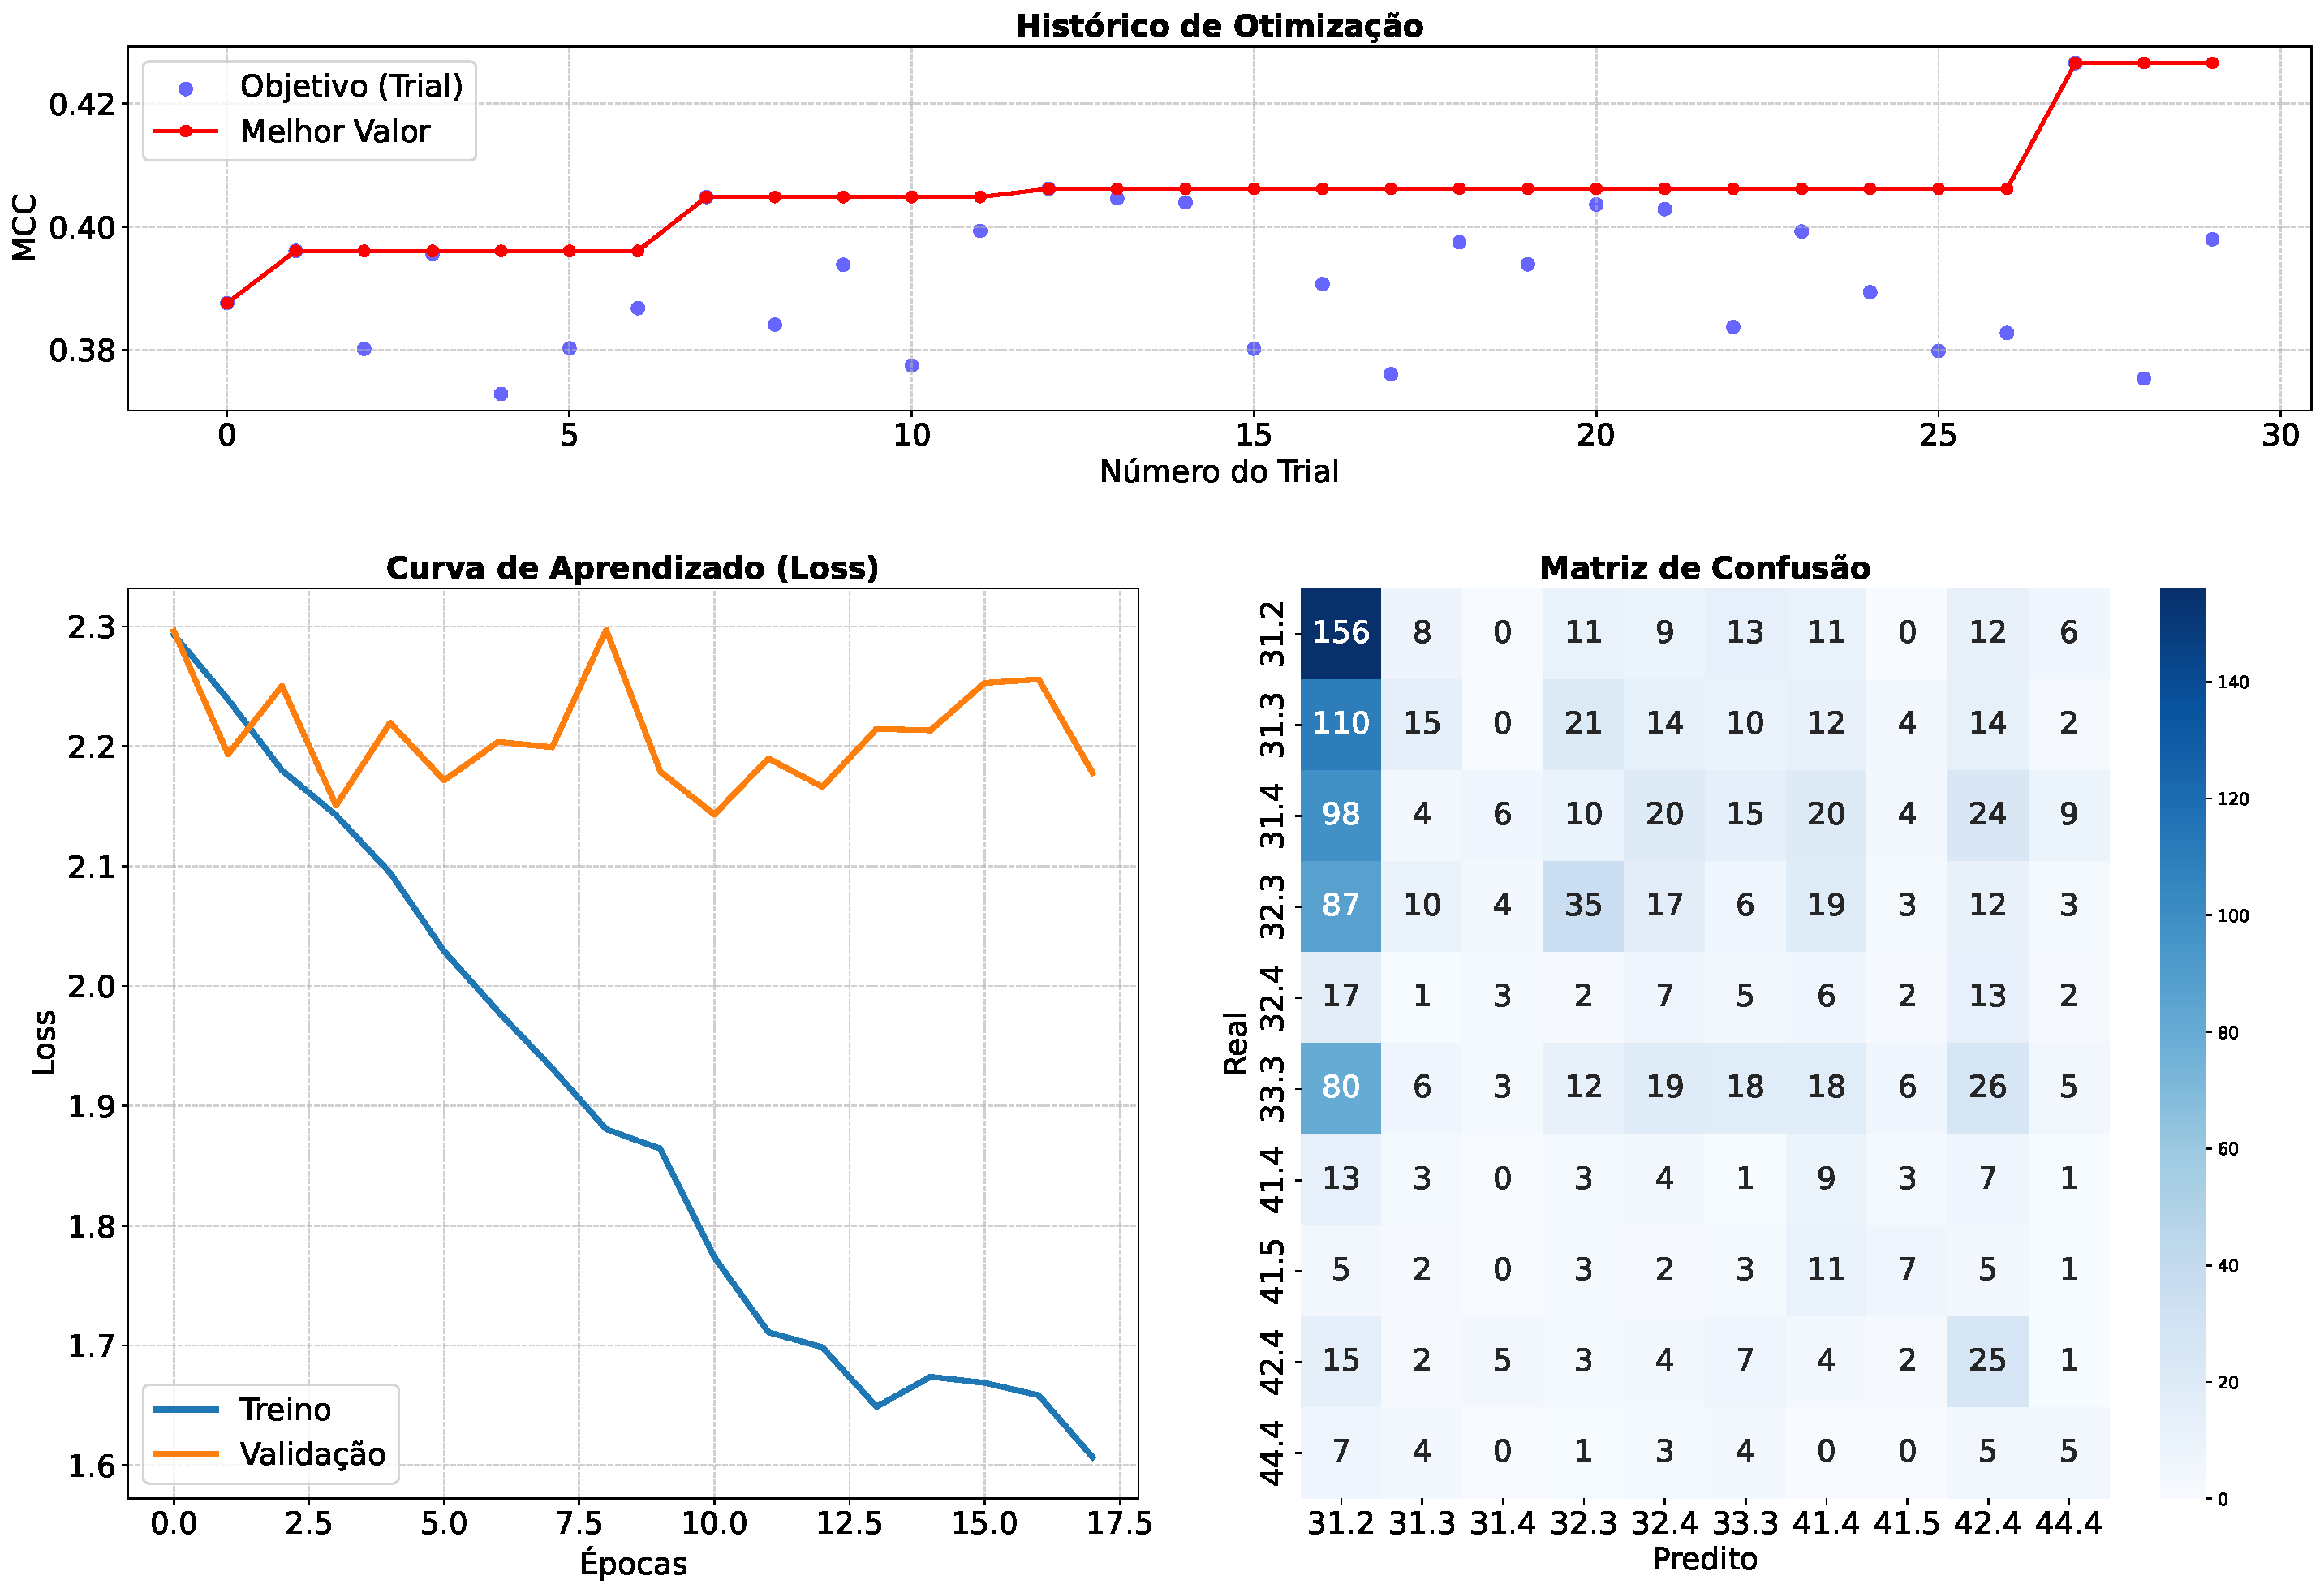
\includegraphics[width=0.85\textwidth]{tex/appendix/experiments/inception_v11_AM_opt_aug/dashboard_consolidado.pdf}
        \caption{Histórico de Otimização, Curvas de Aprendizado e Matriz de Confusão - inception\_v11\_AM\_opt\_aug}
    \end{figure}
\end{minipage}
\clearpage
